%\thispagestyle{empty}
\chapter{Методы численного и натурного исследований} \label{chapt1}

В данной главе будут показаны средства и методы изучения волнения:
\begin{enumerate}
  \item Методы натурных наблюдений (датчики и т.д.). Статья датчики и системы
  \item Методы хранения База данных
  \item Методы Пересчета из придонного давления в обычное
  \item Методы учета влияния нелинейности
\end{enumerate}

\section{Измерители и методы натурных наблюдений}
В настоящем разделе будут рассмотрены основные методы и аппаратные средства регистрации и мониторинга опасных морских явлений, в том числе длинноволновых колебаний в диапазоне цунами. Основное внимание будет уделено морской регистрирующей аппаратуре и сопутствующим техническим средствам, использованным в экспериментальных исследованиях, описанных в данной работе.
\subsection{Обзор современной аппаратуры для измерения волнения в открытом море}
Для измерения гидрофизических параметров в открытом море используется большое число первичных преобразователей – средств измерения, которые предназначены для выработки сигнала измерительной информации в форме, удобной для передачи, дальнейшего преобразования, обработки или хранения, но не поддающейся непосредственному восприятию наблюдателем. Обычно изменение гидрофизического параметра преобразуется в изменение электрического сигнала.

Все измерители можно разделить на несколько групп:
\begin{enumerate}

  \item \textbf{Электродные и емкостные датчики давления}.

      Абзац Струнные датчики
  \item \textbf{Плавающие волнографы}

        Абзац
  \item \textbf{Доплеровские акустические измерители профилей течений}

      Наиболее точными и удобными в использовании в открытом море для измерения волнения являются приборы, принцип измерения которых, основан на  эффекте Допплера. Такой прибор излучает последовательность высокочастотных звуковых импульсов которые отражаются от движущихся в воде частиц и поверхности(примеси, планктон, седименты и т.д.). В зависимости от того движутся частички по направлению от источника звука или к нему, частота отражённого сигнала, принимаемого прибором выше или ниже. Частички движущиеся от инструмента производят сигнал с меньшей частотой и наоборот. Таким прибор точно регистрирует не только смещение водной поверхности, но скорость течений на различных глубинах. Доплеровские акустические измерители устанавливаются под поверхностью моря на дне или на твердом основании. Однако ввиду высокой стоимости, эти приборы пока не нашли повсеместного применения в отечественной океанологии.
  \item \textbf{Радиолокационный метод измерения волнения}

      Абзац
  \item \textbf{Волнограф на базе датчика придонного давления}dfgdfgf
\end{enumerate}


Принципы действия большинства этих средств измерения подробно изложены в литературе \cite{kovalev1993}.

\subsection{Измеритель волнения АРВ-К}

В качестве основного измерителя волнения был выбран прибор разработки ООО СКТБ "Элпа" в основу, которого лежит принцип измерения пульсаций давления, индуцируемых поверхностным волнением в толще моря.

Автономный донный регистратор гидростатического давления выполнен в корпусе из нержавеющей стали и имеет цилиндрическую форму. На рис. \ref{img:ARV} представлена принципиальная конструкция датчика. В качестве первичных преобразователей физических величин используются кварцевые резонаторы. Такой выбор неслучаен: пьезорезонансные элементы имеют малую температурную зависимость и высокую точность. Сигнал с автогенератора, к которому подключены первичные преобразователи, подается на вход регистратора. Регистратор реализован на базе микроконтроллера MSP430 фирмы Texas Instruments. Структурная схема этого регистратора представлена на рис. \ref{img:ARV_regScheme}.

\begin{figure} [h]
  \center
  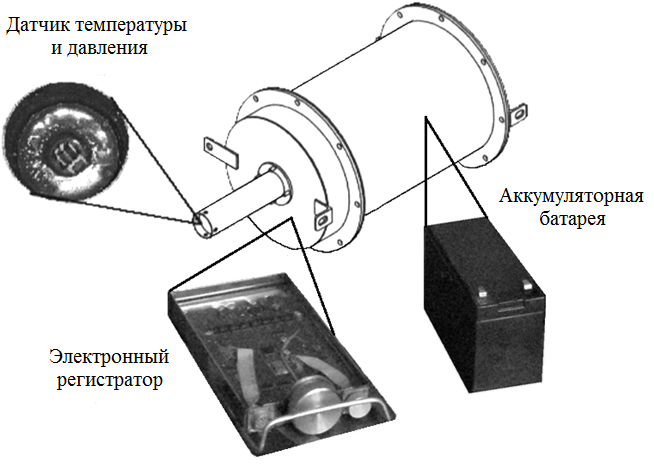
\includegraphics [scale=0.7] {ARV.png}
  \caption{Конструкция автономного регистратора придонного давления АРВ}
  \label{img:ARV}
\end{figure}

Съем частоты с автогенератора производится посредством счетчика–таймера микроконтроллера. Сохранение данных на регистраторе производится на полупроводниковую энергонезависимую память. Значения частоты автогенератора записываются в энергонезависимую память вместе с показаниями системных часов, которые синхронизируются на всех датчиках непосредственно перед постановкой. Полный объем памяти на регистраторе – 64 Мб, чего вполне достаточно для непрерывной регистрации избыточного гидростатического давления в течение 6 месяцев. В конструкции этого регистратора используются элементы питания Delta (12 В). Емкость батарей питания такова, что при текущем энергопотреблении регистратора возможно наращивание как емкости памяти, так и расширение функциональности путем добавления первичных преобразователей других физических величин.

\begin{figure} [h]
  \center
  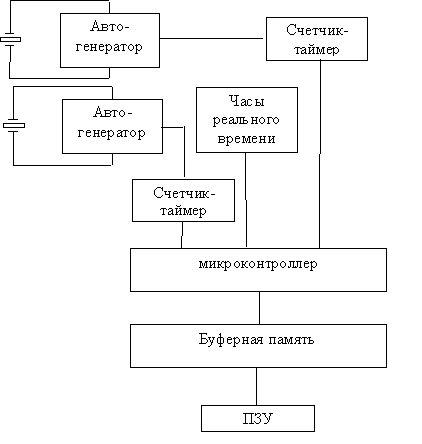
\includegraphics [scale=0.7] {ARV_regScheme.png}
  \caption{Структурная схема регистратора датчика придонного давления и температуры АРВ-К}
  \label{img:ARV_regScheme}
\end{figure}
\FloatBarrier

Характеристики различных моделей Автономного регистратора волнения (АРВ) представлены в таблице \ref{tbl:charact}

\LTXtable{\textwidth}{tblCharact}


\subsubsection{Подробные характеристики из диссера Чернова}
\subsubsection{Схема постановки(как опускается)}




%\newpage
%============================================================================================================================

\section{Формулы} \label{sect1_3}

\subsection{Ненумерованные одиночные формулы} \label{subsect1_3_1}

Вот так может выглядеть формула, которую необходимо вставить в строку по тексту: $x \approx \sin x$ при $x \to 0$.

А вот так выглядит ненумерованая отдельностоящая формула c подстрочными и надстрочными индексами:
$$
(x_1+x_2)^2 = x_1^2 + 2 x_1 x_2 + x_2^2
$$

При использовании дробей формулы могут получаться очень высокие:
$$
  \frac{1}{\sqrt(2)+
  \displaystyle\frac{1}{\sqrt{2}+
  \displaystyle\frac{1}{\sqrt{2}+\cdots}}}
$$

В формулах можно использовать греческие буквы:
$$
\alpha\beta\gamma\delta\epsilon\varepsilon\zeta\eta\theta\vartheta\iota\kappa\lambda\\mu\nu\xi\pi\varpi\rho\varrho\sigma\varsigma\tau\upsilon\phi\varphi\chi\psi\omega\Gamma\Delta\Theta\Lambda\Xi\Pi\Sigma\Upsilon\Phi\Psi\Omega
$$

%\newpage
%============================================================================================================================

\subsection{Ненумерованные многострочные формулы} \label{subsect1_3_2}

Вот так можно написать две формулы, не нумеруя их, чтобы знаки равно были строго друг под другом:
\begin{eqnarray}
  f_W & = & \min \left( 1, \max \left( 0, \frac{W_{soil} / W_{max}}{W_{crit}} \right)  \right), \nonumber \\
  f_T & = & \min \left( 1, \max \left( 0, \frac{T_s / T_{melt}}{T_{crit}} \right)  \right), \nonumber
\end{eqnarray}

Можно использовать разные математические алфавиты:
\begin{eqnarray}
\mathcal{ABCDEFGHIJKLMNOPQRSTUVWXYZ} \nonumber \\
\mathfrak{ABCDEFGHIJKLMNOPQRSTUVWXYZ} \nonumber \\
\mathbb{ABCDEFGHIJKLMNOPQRSTUVWXYZ} \nonumber
\end{eqnarray}

Посмотрим на систему уравнений на примере аттрактора Лоренца:

$$
\left\{
  \begin{array}{rl}
    \dot x = & \sigma (y-x) \\
    \dot y = & x (r - z) - y \\
    \dot z = & xy - bz
  \end{array}
\right.
$$

А для вёрстки матриц удобно использовать многоточия:
$$
\left(
  \begin{array}{ccc}
  	a_{11} & \ldots & a_{1n} \\
  	\vdots & \ddots & \vdots \\
  	a_{n1} & \ldots & a_{nn} \\
  \end{array}
\right)
$$


%\newpage
%============================================================================================================================
\subsection{Нумерованные формулы} \label{subsect1_3_3}

А вот так пишется нумерованая формула:
\begin{equation}
  \label{eq:equation1}
  e = \lim_{n \to \infty} \left( 1+\frac{1}{n} \right) ^n
\end{equation}

Нумерованых формул может быть несколько:
\begin{equation}
  \label{eq:equation2}
  \lim_{n \to \infty} \sum_{k=1}^n \frac{1}{k^2} = \frac{\pi^2}{6}
\end{equation}

В последствии на формулы (\ref{eq:equation1}) и (\ref{eq:equation2}) можно ссылаться.

%\newpage
%============================================================================================================================

\clearpage
